\documentclass{article}

% Encodings, page setup, paragraph formatting, font
\usepackage[top=0.9in, bottom=1in, left=1.5in, right=1.5in]{geometry}
\usepackage[icelandic]{babel}
\usepackage[T1]{fontenc}
\usepackage[sc]{mathpazo}
\usepackage[parfill]{parskip}
\usepackage{cancel}
\usepackage{comment}
% Tables and lists
\usepackage{booktabs,tabularx}
\usepackage{multirow}
\usepackage{enumerate}
\usepackage{adjustbox}
\usepackage{multicol}
\usepackage{enumitem}
\usepackage{xcolor}
% Math
\usepackage{amsmath, amsfonts, amssymb, amsthm}
\usepackage{gensymb}
% Graphics
\usepackage{graphicx}
\usepackage{forest}
\usepackage{tikz}
\usetikzlibrary{positioning, shapes, arrows.meta}
% Code environment
\usepackage{listingsutf8}
\definecolor{commentcolor}{RGB}{0, 128, 0}
\definecolor{keywordcolor}{RGB}{0, 0, 255}
\definecolor{stringcolor}{RGB}{163, 21, 21}
\definecolor{numbercolor}{RGB}{128, 0, 128}
\definecolor{identifiercolor}{RGB}{0, 0, 0}

\lstset{
    language=Java,
    basicstyle=\ttfamily,
    keywordstyle=\color{keywordcolor}\bfseries,
    commentstyle=\color{commentcolor},
    identifierstyle=\color{identifiercolor},
    stringstyle=\color{stringcolor},   
    showstringspaces=false,
    numbers=left,
    numberstyle=\tiny\color{gray},
    tabsize=2,
    breaklines=true,
    columns=fullflexible,
    keepspaces=true,
    inputencoding=utf8, 
    extendedchars=true,  
    literate=
        {á}{{\'a}}1
        {ð}{{\dh}}1
        {é}{{\'e}}1
        {í}{{\'i}}1
        {ó}{{\'o}}1
        {ú}{{\'u}}1
        {ý}{{\'y}}1
        {þ}{{\th}}1
        {æ}{{\ae}}1
        {ö}{{\"o}}1
        {Á}{{\'A}}1
        {Ð}{{\DH}}1
        {É}{{\'E}}1
        {Í}{{\'I}}1
        {Ó}{{\'O}}1
        {Ú}{{\'U}}1
        {Ý}{{\'Y}}1
        {Þ}{{\TH}}1
        {Æ}{{\AE}}1
        {Ö}{{\"O}}1,
}

\title{OOPS (Online Order Printing Software)}
\author{Team 16 - brj46, hfd2, jjo1, ros3}
\date{Haust 2025}

\begin{document}

\maketitle

\vspace{5em}
\begin{center}
    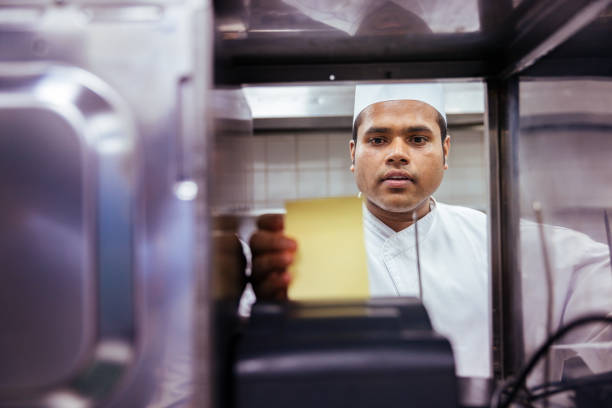
\includegraphics[width=0.8\textwidth]{imgs/order-in-kitchen.jpg}
\end{center}


\newpage

\section{Project Vision}

\subsection{Vision Statement}
To empower businesses to process online orders instantly and accurately, making every transaction seamless and stress-free. The system is designed to remove barriers for both restaurant owners and customers, providing a smooth and reliable experience from order creation to fulfillment.

\subsection{Long-Term Goal}
The long-term vision of this project is to enable restaurant owners to receive and manage orders without the need for direct phone calls or manual input. Customers will be able to place orders online via a mobile app or website, reducing staff workload and minimizing errors.

\subsection{Value for Stakeholders}
\textbf{Customers:} Can browse menus, place orders, see totals, and save favorites. In the beta version, payments will be made at pickup to simplify adoption.\\

\textbf{Restaurant Staff:} Gain a login to manage pending and closed orders, adjust order queue times, and mark items as temporarily sold out.\\

\textbf{Administrators:} Have full control over menus, pricing, and opening hours. They also gain access to sales reports and item popularity analytics, empowering data-driven decisions.

\subsection{Competitive Advantage}
Unlike traditional phone-based ordering or existing delivery platforms that often take a commission, this system gives restaurants direct control over their online orders. With built-in analytics and flexible administration features, it not only streamlines the ordering process but also provides valuable insights into customer behavior and sales trends.

\newpage
\section{Use Case Document}

\subsection*{UC1: Place Order (Pay at Pickup)}
\textbf{Scope:} Restaurant Online Ordering System \\
\textbf{Level:} User goal \\
\textbf{Primary actor:} Customer \\

\textbf{Stakeholders \& interests:}
\begin{itemize}
    \item Customer: Wants to browse menu, create order, see total price, and receive clear pickup time without errors.
    \item Restaurant Staff: Wants accurate, complete orders, and realistic queue times.
    \item Restaurant Owner/Admin: Wants increased order throughput and fewer phone calls; accurate sales and item popularity data.
\end{itemize}

\textbf{Preconditions:}
\begin{itemize}
    \item Menu and opening hours are available.
    \item System is accepting orders.
\end{itemize}

\textbf{Success guarantee:}
\begin{itemize}
    \item Order recorded with items, prices, and total.
    \item Order status set to ``Pending.''
    \item Pickup time estimated.
    \item Customer receives confirmation.
\end{itemize}

\textbf{Main success scenario:}
\begin{enumerate}
    \item System displays current menu.
    \item Customer adds items to basket.
    \item System shows running total and pickup time.
    \item Customer enters phone number.
    \item Customer reviews and confirms order.
    \item System validates store and availability.
    \item System creates order, assigns ID.
    \item System presents confirmation and notifies staff.
\end{enumerate}

\textbf{Extensions / alternate scenarios:}
\begin{itemize}
    \item[(2a)] Item sold out:
    \begin{enumerate}
        \item System notifies customer that the item is unavailable.
        \item Customer either replaces the item or removes it from basket.
    \end{enumerate}

    \item[(4a)] Invalid phone number:
    \begin{enumerate}
        \item System detects phone number does not match valid format.
        \item System requests correction from the customer.
        \item Customer re-enters phone number.
    \end{enumerate}

    \item[(5a)] Store just closed:
    \begin{enumerate}
        \item System checks current store opening hours.
        \item System rejects the order and notifies customer of closure.
    \end{enumerate}

    \item[(6a)] Inventory threshold hit:
    \begin{enumerate}
        \item System detects item availability is below threshold.
        \item System prevents checkout of that item.
        \item Customer edits basket to adjust or remove the item.
    \end{enumerate}

    \item[(7a)] Notification delivery fails:
    \begin{enumerate}
        \item System attempts to send confirmation to customer.
        \item System fails to deliver via chosen channel.
        \item System shows confirmation on screen and logs error.
    \end{enumerate}
\end{itemize}


\textbf{Special requirements:}
\begin{itemize}
    \item Pickup time shown $<$ 1 second after basket update.
    \item Confirmation within 2 seconds.
    \item Accessibility requirements met.
\end{itemize}

\textbf{Technology \& data variations:}
\begin{itemize}
    \item International phone formats supported.
    \item Future: online payments.
    \item Reorder favorites feature possible.
\end{itemize}

\textbf{Frequency:} High during open hours.\\
\textbf{Open issues:} Phone number retention, taxes, notification channels.

\subsection*{UC2: Manage Menu (Add/Update/Remove Items)}
\textbf{Scope:} Restaurant Online Ordering System \\
\textbf{Level:} User goal \\
\textbf{Primary actor:} Admin \\

\textbf{Stakeholders \& interests:}
\begin{itemize}
    \item Admin: Needs control over menu, prices, availability.
    \item Customers: Need accurate menus.
    \item Staff: Wants fewer manual corrections.
\end{itemize}

\textbf{Preconditions:} Admin authenticated.\\
\textbf{Success guarantee:} Menu changes are persisted and reflected. Logged for audit.\\

\textbf{Main success scenario:}
\begin{enumerate}
    \item Admin signs in.
    \item Opens menu management.
    \item Creates or edits item.
    \item Updates properties (name, price, etc.).
    \item System validates inputs.
    \item Admin saves.
    \item System persists changes.
    \item System confirms success.
    \item Customers see update.
\end{enumerate}

\textbf{Extensions / alternate scenarios:}
\begin{itemize}
    \item[(3a)] Remove item with open orders:
    \begin{enumerate}
        \item Admin attempts to delete an item.
        \item System checks if the item is part of any open orders.
        \item If yes, system prevents deletion and notifies admin.
        \item Admin may mark the item as unavailable instead.
    \end{enumerate}

    \item[(5a)] Validation error:
    \begin{enumerate}
        \item System detects invalid input (e.g., empty name, negative price).
        \item System highlights the error field and prompts correction.
        \item Admin corrects and retries save.
    \end{enumerate}

<<<<<<< HEAD
    \item[(6a)] Concurrent edit detected:
    \begin{enumerate}
        \item Another admin is editing the same item at the same time.
        \item System notifies of conflict and provides resolution options.
        \item Admin chooses whether to override or merge changes.
    \end{enumerate}

    \item[(8a)] Cache delay:
    \begin{enumerate}
        \item Customers may not immediately see the updated menu due to caching.
        \item System shows a warning to admin about possible delay.
        \item Updates propagate within a few seconds.
    \end{enumerate}
=======

>>>>>>> origin/main
\end{itemize}


\textbf{Special requirements:}
\begin{itemize}
    \item Audit trail of changes.
    \item Update latency $<$ 5 seconds.
    \item Role-based access control.
\end{itemize}

\textbf{Frequency:} Moderate (weekly/daily).\\
\textbf{Open issues:} Price rounding, image hosting.

\subsection*{UC3: Set Order Queue Time (Adjust Estimated Prep/Wait)}
\textbf{Scope:} Restaurant Online Ordering System \\
\textbf{Level:} User goal \\
\textbf{Primary actor:} Staff/Admin \\

\textbf{Stakeholders \& interests:}
\begin{itemize}
    \item Staff: Needs realistic pickup times.
    \item Customers: Want accurate estimates.
    \item Owner/Admin: Wants fewer cancellations.
\end{itemize}

\textbf{Preconditions:}
\begin{itemize}
    \item Staff authenticated.
    \item Store open.
\end{itemize}

\textbf{Success guarantee:}
\begin{itemize}
    \item Queue time updated.
    \item Applied to new orders.
    \item Logged with timestamp and actor.
\end{itemize}

\textbf{Main success scenario:}
\begin{enumerate}
    \item Staff signs in.
    \item Opens dashboard.
    \item Reviews pending orders.
    \item Adjusts queue time.
    \item System validates bounds.
    \item System applies change.
    \item Confirmation shown.
\end{enumerate}

\textbf{Extensions / alternate scenarios:}
\begin{itemize}
<<<<<<< HEAD
    \item[(4a)] Auto-suggested queue time:
    \begin{enumerate}
        \item System analyzes order volume and historical averages.
        \item System proposes a recommended queue time.
        \item Staff may accept or override the suggestion.
    \end{enumerate}
=======
>>>>>>> origin/main

    \item[(5a)] Out-of-range input:
    \begin{enumerate}
        \item Staff enters a queue time outside valid limits.
        \item System rejects the input and suggests a valid range.
        \item Staff re-enters a valid value.
    \end{enumerate}

<<<<<<< HEAD
    \item[(6a)] Existing orders flagged:
    \begin{enumerate}
        \item Queue time update applies only to new orders.
        \item System flags existing pending orders if discrepancies arise.
        \item Staff reviews flagged orders as needed.
    \end{enumerate}
=======
>>>>>>> origin/main

    \item[(6b)] Scheduled rules override:
    \begin{enumerate}
        \item A scheduled rule (e.g., lunch rush adjustment) is active.
<<<<<<< HEAD
        \item System notifies staff that the manual change is overridden.
        \item Staff may adjust the schedule instead if necessary.
=======
        \item System prompts staff for new queue time during a scheduled rule.
        \item Staff may adjust the schedule if necessary.
>>>>>>> origin/main
    \end{enumerate}
\end{itemize}


\textbf{Special requirements:}
\begin{itemize}
    \item Change applied in $<$ 2 seconds.
    \item All changes traceable.
\end{itemize}

\textbf{Frequency:} Variable, often during peaks.\\
\textbf{Open issues:} Policy on updating existing orders, scheduled vs. ad-hoc overrides.




\paragraph{UC4: View Menu}  
A customer selects a restaurant and the system shows the current menu with categories, item names, descriptions, prices, photos, and real-time availability. Information including photos are uploaded by the restaurant owner and retrieved from the database through an advanced endpoint, ensuring customers see up-to-date visual representations of items. The system ensures only currently available items are shown and reflects temporary “sold out” statuses immediately.

\paragraph{UC5: Sign In (Staff/Admin)}  
A staff member or admin provides credentials; the system authenticates and grants access to role-appropriate features (orders dashboard for staff; menu and reports for admin). Failed attempts are limited and logged; on success, the user is taken to the relevant workspace.

\paragraph{UC6: View Sales Report}  
An admin opens the reporting section and selects a date range. The system aggregates sales totals, average order value, item-level popularity, and trends. The admin can export results and use insights to adjust prices, menu, or staffing.

\paragraph{UC7: Adjust Opening Hours and Exceptions (Admin)}  
An admin updates regular opening hours and sets one-time exceptions such as holidays or early closures. The system validates the new schedule, applies the changes to ordering eligibility, and ensures customers cannot place orders outside the adjusted hours.

\paragraph{UC8: Manage Roles and Access (Admin)}  
An admin assigns or revokes roles (Staff, Admin) for other users. The system updates access permissions immediately, ensuring that each user can only access features appropriate to their role. All role changes are logged for security and accountability.

\paragraph{UC9: View Order Status (Customer)}  
A customer enters their order ID (and optionally phone number) to check the current status of their order. The system shows whether it is Pending, Preparing, Ready, or Closed, along with the estimated pickup time.

\paragraph{UC10: Set Order Status (Staff)}  
A staff member updates the status of an order, such as moving it from Pending to Preparing, from Preparing to Ready, and finally to Closed once picked up. The system records each update, ensures proper sequence of states, and notifies the customer if applicable.


\section{Project Estimation and Prioritization}

We use a \textbf{grouped priority system} where a lower number means higher priority (P1 > P2 > P3).
Time estimates are in \textbf{person hours}.
\begin{center}
\begin{adjustbox}{max width=\textwidth}
\begin{tabular}{|l|c|c|}
\hline
\textbf{Use Case} & \textbf{Time Estimation (hours)} & \textbf{Priority} \\ \hline
UC1: Place Order (Pay at Pickup)                 & 10 & P0 \\ \hline
UC2: Manage Menu                                 & 15 & P0 \\ \hline
UC3: Set Order Queue Time                        & 12 & P1 \\ \hline
UC4: View Menu                                   & 5  & P0 \\ \hline
UC5: Sign In (Staff/Admin)                       & 6  & P1 \\ \hline
UC6: View Sales Report                           & 8  & P1 \\ \hline
UC7: Adjust Opening Hours \& Exceptions (Admin)  & 6  & P2 \\ \hline
UC8: Manage Roles \& Access (Admin)              & 6  & P2 \\ \hline
UC9: View Order Status (Customer)                & 5  & P1 \\ \hline
UC10: Set Order Status (Staff)                   & 6  & P1 \\ \hline
\end{tabular}
\end{adjustbox}
\end{center}

\section{Project Plan and Schedule}

The project spans \textbf{10 weeks} with 4 sprints (Sprint 1: 2 weeks, Sprint 2: 3 weeks, Sprint 3: 3 weeks, Sprint 4: 2 weeks).
Each sprint has a designated Product Owner (P.O.).

\begin{center}
\renewcommand{\arraystretch}{1.6} % row height
\large % larger font
\begin{adjustbox}{max width=\textwidth}
\begin{tabular}{|c|>{\raggedright\arraybackslash}p{5cm}|c|c|c|>{\raggedright\arraybackslash}p{4cm}|}
\hline
\textbf{Week} & \textbf{Use Cases / Activities} & \textbf{Expected Hours} & \textbf{P.O.} & \textbf{Sprint} & \textbf{Consultation} \\ \hline
1  & None -- setup \& planning                    & \textasciitilde5  & BRJ & 1 & \textbf{A1 Presentation} \\ \hline
2  & UC1: Place Order; Android skeleton           & \textasciitilde20 & BRJ & 1 & Model Drafts \\ \hline
3  & UC2: Manage Menu; UC3: Set Queue Time        & \textasciitilde25 & JJO & 2 & \textbf{A2 Presentation} \\ \hline
4  & UC4: View Menu; UC5: Sign In; UC6: Reports   & \textasciitilde20 & JJO & 2 & Dev support \\ \hline
5  & Testing UC1--UC6; integration                & \textasciitilde15 & JJO & 2 & Dev support \\ \hline
6  & UC7: Opening Hours; UC8: Roles; UC9: Order Status (Cust); UC10: Order Status (Staff) & \textasciitilde20 & HFD & 3 & \textbf{A3 Presentation} \\ \hline
7  & Scaling improvements; performance checks     & \textasciitilde15 & HFD & 3 & Dev support \\ \hline
8  & Final features; Print orders                & \textasciitilde15 & HFD & 3 & Dev support \\ \hline
9  & Final testing; bug fixes                     & \textasciitilde20 & ROS & 4 & A4 Prep \\ \hline
10 & Delivery; deployment; presentation           & \textasciitilde15 & ROS & 4 & Final Presentation \\ \hline
\end{tabular}
\end{adjustbox}
\end{center}


\section{Project Skeleton}

\textbf{GitHub Repository:} \texttt{https://github.com/Reynirjr/Hugbo1-team16}

\textbf{Team Members and Accounts:}
\begin{itemize}
    \item BRJ -- \texttt{Reynirjr}
    \item JJO -- \texttt{jonnishmurda}
    \item HFD -- \texttt{helgarfri}
    \item ROS -- \texttt{Robertorri}
\end{itemize}

All team members have access and have made at least one commit (e.g., updating the README, adding skeleton files, or first endpoints).  
The skeleton was generated using \textbf{Java Spring} and uploaded to GitHub for collaborative development.


\end{document}


